\appendix
\section{Démonstrations}

\subsection{Lemmes}

\begin{lemme}[Décision neutre au risque]
  \label{lem:ndef}
  La solution au problème
  \begin{equation}
    \maximizeEquation[q \in \Q]{\hEN(q) - \frac{\lambda}{2}\|q\|^2}
  \end{equation}
  est donnée par
  \begin{equation}
    \qh_1 = \frac{1}{n\lambda}\sumi r_i|x_i\rangle.
  \end{equation}
  On en déduit par ailleurs que
  \begin{equation}
    \hEN = \lambda\langle\qh_1|
  \end{equation}
  et donc que
  \begin{equation}
    \hEN(\qh_1) = \lambda\|\qh_1\|^2
  \end{equation}
  et
  \begin{equation}
    \hEN_\lambda(\qh_1) = \frac{\lambda}{2}\|\qh_1\|^2.
  \end{equation}
\end{lemme}

\begin{proof}
  Si on considère un déplacement de décision $\qh_1 + \Delta q$, alors par linéarité le premier
  terme de l'objectif devient $\hEN(\qh_1+\Delta q) = \hEN(\qh_1) + \hEN(\Delta q)$ et le terme de
  régularisation devient 
  \begin{equation}
    -\lambda/2\|\qh_1 + \Delta q\|^2 = -\lambda/2\|\qh_1\|^2 - \lambda\braket{\qh_1|\Delta q} - \lambda/2\|\Delta q\|^2.
  \end{equation}
  On a donc
  \begin{align}
    \hEN_\lambda(\qh_1)  - \hEN_\lambda(\qh_1+\Delta q) &= -\hEN(\Delta q) + \lambda\braket{\qh_1|\Delta q} + \lambda/2\|\Delta q\|^2\\
                                       &= -\lambda\braket{\qh_1|\Delta q} + \lambda\braket{\qh_1|\Delta q} +
                                         \lambda/2\|\Delta q\|^2\\
                                       &= \lambda/2\|\Delta q\|^2 \geq 0,
  \end{align}
  Ce qui entraîne $\hEN_\lambda(\qh_1) \geq \hEN_\lambda(\qh_1 + \Delta q)$ pour tout déplacement $\Delta q\in\Q$. 
\end{proof}


\begin{lemme}[Forte concavité de l'objectif]
  \label{lem:conv}
  Soit $\S_n$ un ensemble d'entraînement et $\qh = \argmax\EU_\lambda(q)$ la décision
  régularisée optimale. Alors pour toute décision $q \in \Q$,
  \begin{equation}
    \frac{\lambda}{2}\|\qh - q\|^2 \leq \hEU_\lambda(\qh) - \hEU_\lambda(q).
  \end{equation}
\end{lemme}

\begin{lemme}[Sigma admissibilité]
  \label{lem:sig}
  Soit $q,q' \in \Q$ deux vecteurs de décision et $(x,r) \in \M$ deux points quelconques du
  support de la loi de marché. Alors
  \begin{equation}
    |u(r\,q(x)) - u(r\,q'(x))| \leq \gamma\rmax\xi\|q-q'\|.
  \end{equation}
\end{lemme}

\begin{proof}
  D'abord avec la propriété Lipschitz de $u$ puis par l'hypothèse $|r|\leq\rmax$, on obtient
  \begin{align}
    |u(r\,q(x)) - u(r\,q'(x))| &\leq \gamma\rmax|(q(x) - q'(x))|.\\
    \intertext{Puis en notation vectorielle on obtient}
                               &=\gamma\rmax|\braket{q|x} - \braket{q'|x}|\\
                               &=\gamma\rmax|\langle q-q'|x \rangle|\\
                               &\leq\gamma\rmax\xi\|q-q'\|
  \end{align}
  successivement par Cauchy Schwartz et par l'hypothèse $\kappa(x,x)\leq\xi$, ce qui complète la
  démonstration.
\end{proof}

\begin{lemme}[Stabilité]
  \label{lem:stab}
  Soit $\S_n$ et $S_n'$ deux ensembles d'entraînement ne différant qu'à leur $j$\ieme
  point:
  \begin{align}
    \S_n &= \{(x_1,r_1),\ldots,(x_j,r_j),\ldots,(x_n,r_n)\}\\
    \S_n' &= \{(x_1,r_1),\ldots,(x'_j,r'_j),\ldots,(x_n,r_n)\},
  \end{align}
  et soit $\qh = \alg(\S_n)$ et $\qh' = \alg(\S_n')$ les deux décisions optimales
  correspondantes. Alors
  \begin{equation}
    \|\qh - \qh'\| \leq \frac{2\gamma\xi\rmax}{\lambda n}.
  \end{equation}
\end{lemme}

\begin{rem}
  Cette propriété a été démontrée par \cite{bousquet2002stability}. Nous en donnons ici
  une version simplifiée et adaptée à la situation. Voir aussi \cite{mohri2012foundations}
  pour une démonstration dans un contexte général.
\end{rem}

\begin{proof}
  Posons $\hEU = \hEU(\S_n,\cdot)$ et $\hEU' = \hEU(\S_n',\cdot)$. Du Lemme \ref{lem:conv}, on
  obtient
  \begin{equation}
    \lambda\|\qh - \qh'\|^2 \leq \hEU_\lambda(\qh) - \hEU_\lambda(\qh') + \hEU'_\lambda(\qh') - \hEU'_\lambda(\qh).
  \end{equation}
  Les termes de régularisation s'annulent et on obtient donc:
  \begin{equation}
    \lambda\|\qh - \qh'\|^2 \leq \hEU(\qh) - \hEU(\qh') + \hEU'(\qh') - \hEU'(\qh)
  \end{equation}
  Ces deux différences font disparaître tous les termes, excepté le
  $j$\ieme:
  \begin{align}
    \lambda\|\qh - \qh'\|^2 \leq &\,n^{-1}(u(r_j\qh(x_j)) - u(r_j\qh'(x_j)))\, + \\
                        & \qquad n^{-1}(u(r_j'\qh'(x_j')) - u(r_j'\qh'(x_j'))).
  \end{align}
  D'autre part, cette somme est positive par le terme de gauche, on peut donc
  successivement appliquer l'opérateur valeur absolue, l'inégalité du triangle et
  le résultat du Lemme \ref{lem:sig} pour obtenir
  \begin{equation}
    \lambda\|\qh - \qh'\|^2 \leq \frac{2}{n}\gamma\rmax\xi\|\qh - \qh'\|,
  \end{equation}
  d'où on tire le résultant annoncé.
\end{proof}

\begin{lemme}[Décision limite]
  \label{lem:dl}
  Soit $\S_n$ un ensemble d'entraînement, $\qh_u = \argmax_q\hEU_\lambda(q)$ la solution au
  problème pour une utilité $u$ quelconque (respectant les hypothèses) et
  $\qh_1 = \argmax_q\hEN_\lambda(q)$ la solution au problème risque neutre. Alors
  \begin{equation}
    \|\qh_u\| \leq \|\qh_1\| \leq \frac{\rmax\xi}{\lambda}.
  \end{equation}
\end{lemme}

\begin{proof}
  D'abord, par la propriété de forte concavité de $\hEU_\lambda(\qh_u)$ (Lemme \ref{lem:conv}),
  en posant $q=0$, on obtient, $\frac{\lambda}{2}\|\qh_u\|^2 \leq \hEU_\lambda(\qh_u)$, ou encore
  $\lambda\|\qh_u\|^2 \leq \hEU(\qh_u)$.

  On a par ailleurs,
  \begin{equation}
    \hEU(\qh_u) \leq u\big(\hEN(\qh_u)\big) \leq \hEN(\qh_u)
  \end{equation}
  en appliquant successivement l'inégalité de Jensen et l'inégalité $u(x) \leq x$. Ainsi, en
  appliquant Cauchy Schwartz et le résultat du Lemme \ref{lem:ndef},
  \begin{equation}
    \lambda\|\qh_u\|^2 \leq \hEN(\qh_u) =  \lambda\langle\qh_1|\qh_u\rangle \leq \lambda\|\qh_1\|\|\qh_u\|
  \end{equation}
  pour obtenir $\|\qh_u\| \leq \|\qh_1\|$. On obtient la deuxième inégalité simplement avec
  la définition de $\qh_1 = \lambda^{-1}\sumi r_i|x_i\rangle$ et en appliquant les hypothèses
  $r_i\leq\rmax$ et $|x_i\rangle \leq \xi$.
\end{proof}

\begin{lemme}[Domaine d'utilité limite]
  \label{lem:domu}
  Soit $\qh = \alg(\S_n)$ et $\qh = \alg(\S_n')$ deux décision obtenues à partir de deux
  ensembles d'entraînement $\S_n,S_n' \sim M^n$, et soit $(x,r),(x',r') \in \M$ deux points du
  domaine de marché. Alors
  \begin{equation}
    |u(r\,q(x)) - u(r'\,q'(x'))| \leq \lambda^{-1}(\gamma+1)\rmax^2\xi^2.
  \end{equation}
\end{lemme}

\begin{proof}
  Du Lemme \ref{lem:dl} et par hypothèse, on sait que pour tout $(x,r) \in \M$,
  $|r\,\qh(x)| \leq \lambda^{-1}\rmax^2\xi^2$. De plus, $u(x)\leq x$ sur tout le domaine de
  $u$ et $\gamma x \leq u(x)$ si $x<0$ par hypothèse Lipschitz. On en déduit donc que
  \begin{equation}
    \lambda^{-1}\gamma\rmax^2\xi^2 \leq u(r\,\qh(x)) \leq \lambda^{-1}\rmax^2\xi^2.
  \end{equation}
  Donc au plus, deux valeurs d'utilité ne peuvent différer que de $\lambda^{-1}(\gamma+1)\rmax^2\xi^2$.
\end{proof}

\begin{lemme}[Théorème de McDiarmid]
  \label{lem:mcdiarmid}
  Soit $\S_n$ et $\S_n'$ deux ensembles d'entraînement échantillonés à partir d'une
  quelconque variable aléatoire réelle $D$ supportée par $\bm D$ et ne
  différant que d'un seul point, et soit $g:{\bm D}^n\to\Re$ telle que
  \begin{equation}
    |g(\S_n) - g(\S_n')| \leq c.
  \end{equation}
  Alors pour tout $\epsilon>0$ et pour tout échantillon aléatoire $\S_n \sim D^n$,
  \begin{equation}
    \pp\{g(\S_n) - \E g(\S_n) \geq \epsilon\} \leq \exp\left(-\frac{2\epsilon^2}{nc^2}\right).
  \end{equation}
\end{lemme}

\begin{rem}
  De façon équivalente, en posant
  \begin{equation}
    \delta = \exp\left(-\frac{2\epsilon^2}{nc^2}\right),
  \end{equation}
  alors on aura, avec probabilité au moins $1-\delta$, $g(\S_n) < \epsilon + \E g(\S_n)$. Autrement
  dit, avec probabilité au moins $1-\delta$, l'évènement suivant aura lieu:
  \begin{equation}
    g(\S_n) \leq \E g(\S_n) + \sqrt{\frac{nc^2\log(1/\delta)}{2}}.
  \end{equation}
\end{rem}

\begin{proof}
  Consulter \cite{mohri2012foundations} ou \cite{boucheron2013concentration}.
\end{proof}

\subsection{Théorèmes 1 et 2}

\paragraph{Théorème 1.} On rappelle qu'on veut démontrer que pour tout ensemble
d'entraînement, avec probabilité $1-\delta$, 
\begin{equation}
  \zeta(\S_n) = \EU(\alg(\S_n)) - \hEU(\S_n,\alg(\S_n)) \leq \Omega_u.
\end{equation}

\begin{proof}
  L'idée est en fait d'appliquer le théorème de McDiarmid (énoncé au Lemme
  \ref{lem:mcdiarmid}) à l'erreur de généralisation $\hat\zeta(\S_n)$. Pour ce faire, on va
  donc d'abord chercher à borner la différence d'erreur entraînée par deux fonctions de
  décision $\qh = \alg(\S_n)$ et $\qh' = \alg(\S_n')$, où $\S_n$ et $\S_n$ ne diffèrent
  que d'un seul point qu'on supposera être le $j$\ieme.

  Formellement, si on pose
  \begin{align}
    \S_n &= \{(x_1,r_1),\ldots,(x_j,r_j),\ldots,(x_n,r_n)\}\\
    \S_n' &= \{(x_1,r_1),\ldots,(x'_j,r'_j),\ldots,(x_n,r_n)\}.
  \end{align}
  Alors
  \begin{align}
    |\hat\zeta(\qh) - \hat\zeta(\qh')| &= |\EU(\qh) - \hEU(\qh) -\EU(\qh') + \hEU'(\qh')|\\
                               &\leq |\EU(\qh) - \EU(\qh')| + |\hEU(\qh) - \hEU'(\qh')|\label{eq:wtv1}
  \end{align}
  Par le théorème de Jensen appliqué à la fonction valeur absolue, on obtient du premier
  terme que
  \begin{align}
    |\EU(\qh) - \EU(\qh')| &= |\E(u(R\cdot\qh(X)) - u(R\cdot\qh'(X)))|\\
                           &\leq \E|u(R\cdot\qh(X)) - u(R\cdot\qh'(X))|\\
                           &\leq \gamma\rmax\xi\|\qh-\qh'\|\\
                           &\leq \frac{2\gamma^2\rmax^2\xi^2}{\lambda n},
  \end{align}
  en appliquant successivement les Lemmes \ref{lem:sig} et \ref{lem:stab}. Quant au
  deuxième terme de \eqref{eq:wtv1} on peut le borner de la façon suivante:
  \begin{align}
    &|\hEU(\qh) - \hEU'(\qh')|\nonumber\\
    &\qquad = \frac{1}{n}\bigg|u(r_j\qh(x_j)) - u(r_j'\qh'(x_j')) + \sum_{\substack{i=1\\i\neq
    j}}^n\big(u(r_i\qh(x_i)) - u(r_i\qh'(x_j))\big)\bigg|,
  \end{align}
  qu'on peut décomposer en deux termes en appliquant l'inégalité du triangle. Le premier
  terme:
  \begin{equation}
    n^{-1}|u(r_j\qh(x_j)) - u(r_j'\qh'(x_j'))| \leq \frac{(\gamma+1)\rmax^2\xi^2}{\lambda n}
  \end{equation}
  en appliquant le résultat du Lemme \ref{lem:domu}. En appliquant une deuxième fois les
  Lemmes \ref{lem:sig} et \ref{lem:stab}, le deuxième terme est borné par
  \begin{equation}
    \frac{1}{n}\bigg|\sum_{\substack{i=1\\i \neq j}}^n\big(u(r_i\qh(x_i)) -
    u(r_i\qh'(x_j))\big)\bigg| \leq \frac{n-1}{n}\frac{2\gamma^2\rmax^2\xi^2}{\lambda n} \leq \frac{2\gamma^2\rmax^2\xi^2}{\lambda n}.
  \end{equation}

  Une fois toutes réunies, ces inégalités donnent donc
  \begin{align}
    |\hat\zeta(\qh) - \hat\zeta(\qh')| &\leq \frac{2\gamma^2\rmax^2\xi^2}{\lambda n} + \frac{(\gamma+1)\rmax^2\xi^2}{\lambda n}
                                 + \frac{2\gamma^2\rmax^2\xi^2}{\lambda n}\\
                               & = \frac{(4\gamma^2 + \gamma + 1)\rmax^2\xi^2}{\lambda n}.
  \end{align}

  On peut alors directement appliquer le corrolaire du Théorème de McDiarmid (Lemme
  \ref{lem:mcdiarmid}). On trouve donc qu'avec probabilité au moins $1-\delta$, on aura
  \begin{equation}
    \hat\zeta(\S_n) \leq \E\hat\zeta(\S_n) + \frac{(4\gamma^2 + \gamma +
      1)\rmax^2\xi^2}{\lambda}\sqrt{\frac{\log(1/\delta)}{2n}} 
  \end{equation}

  \todo{Mais},
  \begin{equation}
    \hat\zeta(\S_n) \leq \frac{2\gamma\rmax^2\xi^2}{\lambda n}
  \end{equation}
  et donc,
  \begin{equation}
    \hat\zeta(\S_n) \leq \frac{2\gamma\rmax^2\xi^2}{\lambda n} + \frac{(4\gamma^2 + \gamma +
        1)\rmax^2\xi^2}{\lambda}\sqrt{\frac{\log(1/\delta)}{2n}}
  \end{equation}
\end{proof}
ce qui correspond au résultat annoncé.


\clearpage
\newpage










\todo{Ordonner les lemmes selon l'ordre dans lequel ils sont invoqués.}



\begin{lemme}[Borne sur la décision algorithmique]
  \label{lem:bqhat}
  On va ici démontrer que la décision $\hat q(x)$ est bornée, et ce, pour tout $x \in \X$ et
  pour toute solution $\hat q$ de
  \begin{equation}
    \label{b:l1}
    \maximizeEquation[q \in \Q]{\hEU_\lambda(q).}
  \end{equation}
  Pour ce faire, on va mettre à profit la propriété reproductive de $\Q$ induite par
  $\kappa$ qui stipule que
  \begin{equation}
    q(x) = \langle q, \kappa(x,\cdot)\rangle_{\Q} \leq\nq{q}\,\sqrt{\kappa(x,x)},
  \end{equation}
  où l'inégalité découle de l'inégalité Cauchy-Schwartz appliquée au produit interne de
  $\Q$.  On rappelle que, par hypothèse, $\forall x\in\X, \kappa(x,x) \leq \xi^2$; il suffit donc de borner
  $\nq{q}$. De plus, par le Lemme \ref{lem:rn}, il suffit en fait de borner la solution de
  $\hEN_\lambda(q)$. Mais,
  \begin{align}
    \hEN_\lambda(q) &= n^{-1}\sumi r_i\,q(x_i) - \lambda\nq{q}^2\\
              & \leq n^{-1}\sumi r_i\sqrt{\kappa(x_i,x_i)}\nq{q} - \lambda\nq{q}^2\\
              & \leq \rmax \xi \nq{q} - \lambda\nq{q}^2.
  \end{align}
  Puisque l'expression $\rmax \xi \nq{q} - \lambda\nq{q}^2$ est quadratique, elle atteint son
  maximum à
  \begin{equation}
    \nq{q} = \frac{\rmax \xi}{2\lambda},
  \end{equation}
  on en conclut que $\nq{\hat q} \leq (2\lambda)^{-1}\rmax\xi$ et donc que
  \begin{equation}
    \hat q(x) \leq \frac{\rmax\xi^2}{2\lambda}.
  \end{equation}
\end{lemme}



\begin{lemme}[Forte concavité]
  L'objectif est fortement concave, que ce soit sous sa version statistique $\hEU_\lambda$ ou
  probabiliste $\EU_\lambda$. Autrement dit, pour tout $\alpha \in [0,1]$, on a
  \begin{equation}
    \EU_\lambda(tq_1 + (1-\alpha )q_2) \geq \alpha \EU_\lambda(q_1) + (1-\alpha)\EU_\lambda(q_2) + \lambda \alpha(1-\alpha)\nq{q_1-q_2}^2,
  \end{equation}
  et de même pour $\hEU_\lambda$. Effectivement, puisque $u$ est concave et $\nq{\cdot}^2$ est
  convexe, on a successivement:
  \begin{align}
    & \EU_\lambda(\alpha q_1 + (1-\alpha )q_2)\\
    &\qquad= \E u(R\cdot (\alpha q_1+(1-\alpha )q_2)(X)) - \lambda\nq{\alpha q_1 + (1-\alpha)q_2}^2\\
    &\qquad= \E u(\alpha (R\cdot q_1(X)) + (1-\alpha )(R\cdot q_2(X)))- \lambda\nq{\alpha q_1 + (1-\alpha)q_2}^2\\
    &\qquad\geq \E(\alpha  u(R\cdot q_1(X)) + (1-\alpha )u(R\cdot q_2(X))) - \lambda\nq{\alpha q_1 + (1-\alpha)q_2}^2\\
    &\qquad= \alpha\EU(q_1) + (1-\alpha)\EU(q_2) - \lambda\nq{\alpha q_1 + (1-\alpha)q_2}^2\\
    &\qquad= \alpha\EU_\lambda(q_1) + (1-\alpha)\EU_\lambda(q_2) - \lambda(\nq{\alpha q_1+(1-\alpha)q_2}^2 - \alpha\nq{q_1}^2 -
      (1-\alpha)\nq{q_2}^2).
  \end{align}
  Mais d'autre part,
  \begin{align}
    &-\lambda\nq{\alpha q_1 + (1-\alpha)q_2}^2 + \lambda\alpha\nq{q_1}^2+\lambda(1-\alpha)\nq{q}^2\\
    &\qquad = \lambda\alpha(1-\alpha)(\nq{q_1}^2 + \nq{q_2}^2 - 2\langle q_1,q_2\rangle)\\
    &\qquad = \lambda\alpha(1-\alpha)\nq{q_1-q_2}^2,
  \end{align}
  Ce qui complète la démonstration. La dérivation demeure exactement la même lorsqu'on
  considère $\hEU_\lambda$.
\end{lemme}


\begin{lemme}[Borne sur l'équivalent certain]
  \label{lem:ce}
  Soient $\nCE_1 = u^{-1}(\nEU_1)$ et $\nCE_2 = u^{-1}(\nEU_2)$ et soit une borne $\Omega_u$ telle
  que
  \begin{equation}
    \nEU_1 \geq \nEU_2 - \Omega_u.
  \end{equation}
  Par définition du sur-gradient, pour tout $r \in \Re$,
  $u(r+\Delta) \leq u(r) + \Delta\cdot\partial u(r)$. Donc en posant
  $\Delta = \nCE_1 - \nCE_2$ et $r=\nCE_2$, on obtient ces deux inégalités:
  \begin{equation}
    -\Omega_u \leq \nEU_1 - \nEU_2 = u(\nCE_1) - u(\nCE_2) \leq \partial u(\nCE_2)(\nCE_1 - \nCE_2).
  \end{equation}
  On trouve ainsi:
  \begin{equation}
    \nCE_1 \geq \nCE_2 - \Omega_u\cdot \partial u^{-1}(\nCE_2).
  \end{equation}
  Typiquement, $\nCE_1$ et $\nEU_1$ seront des quantités inobservables, alors que $\nCE_2$
  et $\nEU_2$ seront des quantités calculables. De plus, si $\partial u^{-1}(\nCE_2)$ comporte
  plusieurs éléments (\eg\ si la dérivée de $u$ est discontinue à $\nCE_2$), on choisira
  l'élément le plus favorable; la plupart du temps ce sera équivalent à
  $\lim_{r\to\nCE_2^{-}}1/u'(r)$ dans la région où $1/u'(r)$ est défini. Enfin, on note que
  cette limite existe puisque $u$ est strictement monotone, et donc sa pente ne s'annule
  nulle part.
\end{lemme}


\begin{lemme}[Généralisation du lemme de Hoeffding]
  \label{b:lem:hoeffding}
  Ce lemme généralise le lemme de Hoeffding à un espace vectoriel de dimension arbitraire
  $\Q$. Soit un vecteur aléatoire $Q\in\Q$ tel que $\nq{Q}\leq\beta$ et $\E Q = 0$. Alors pour tout
  $t\in\Q$, 
  \begin{equation}
    \E e^{\inp{t,Q}} \leq \exp\left(\frac{\beta^2\|t\|^2}{2}\right).
  \end{equation}
  En effet, on sait que par définition de la convexité de la fonction exponentielle, pour
  tout $s\in[0,1]$,
  \begin{equation}
    \exp(sa + (1-s)b) \leq s\exp a + (1-s)\exp b.
  \end{equation}
  Donc en définissant $g:\{q \in \Q:\|q\|\leq\beta\}\to[0,1]$ par
  \begin{equation}
    g(q) = \frac{1}{2}\left(\frac{\inp{t,q}}{\beta\|t\|} + 1\right)
  \end{equation}
  et en posant $a = \beta\|t\|$ et $b = -\beta\|t\|$, alors pour tout $q \in \Q$,
  \begin{gather}
    a g(q) = \frac{1}{2}(\inp{t,q} + \beta\|t\|),\\
    b (1-g(q)) = - \frac{1}{2}(\beta\|t\| - \inp{t,q}),
  \end{gather}
  et donc
  \begin{equation}
    \exp(ag(q) + (1-g(q))b) = e^{\inp{t,q}}.
  \end{equation}
  La branche droite de l'inégalité devient quant à elle
  \begin{equation}
    \left(\frac{\inp{t,q}}{\beta\|t\|} + 1\right)e^{\beta\|t\|} + \left(1-\frac{\inp{t,q}}{\beta\|t\|}\right)e^{-\beta\|t\|}
  \end{equation}
  et donc, puisque $\E\inp{t,Q} = \inp{t,\E Q} = 0$, 
  \begin{align}
    \E e^{\inp{t,Q}} &\leq \E\left(\left(\frac{\inp{t,Q}}{\beta\|t\|} + 1\right)e^{\beta\|t\|} +
                       \left(1-\frac{\inp{t,Q}}{\beta\|t\|}\right)e^{-\beta\|t\|}\right)\\
                     &= e^{\beta\|t\|} + e^{-\beta\|t\|}\\
                     &= e^{\phi(\beta\|t\|)}
  \end{align}
  où $\phi(x) = \log(e^{x} + e^{-x})$. Or, avec le résultat de \cite{mohri2012foundations},
  p.~370, on a $\phi(x) \leq x^2/2$, d'où on tire le résultat annoncé.
\end{lemme}

\begin{lemme}[Généralisation de la borne de Chernoff]
  \label{b:lem:chernoff}
  Ce lemme généralise la borne de Chernoff à un espace vectoriel de dimension arbitraire
  $\Q$. Soit un vecteur aléatoire $Q \in \Q$. Alors l'évènement $\|Q\| \geq \epsilon$ aura lieu si et
  seulement s'il existe $t \in \Q$, $\|t\|=1$ tel que $\inp{t,Q} \geq \epsilon$. Ainsi, pour tout
  $s>0$, en employant l'inégalité de Markov, 
  \begin{align}
    \pp\{\|Q\| \geq \epsilon\} &= \pp\{s\inp{t,Q} \geq s\epsilon\} = \pp\{e^{s\inp{t,X}} \geq e^{s\epsilon}\}\\
                     &\leq e^{-s\epsilon}\E e^{\inp{t,Q}}.
  \end{align}
\end{lemme}

\begin{lemme}[Généralisation de l'inégalité de McDiarmid]
  \label{b:lem:mcdiarmid}
  L'inégalité de McDiarmid peut également se généraliser à des fonctions prenant leurs
  valeurs dans des espaces vectoriels À élaborer!

  Soit une distribution $\mathscr{F}$ à valeur dans un espace quelconque $\bm F$, un
  espace vectoriel $\Q$ et une fonction $f:\bm F^n\to \Q$. S'il existe une constante
  $c\in\Re$ telle que pour deux ensembles d'échantillons \iid\ $\S_n \sim \mathscr{F}^n$ et
  $\S'_n$, où $\S_n$ et $\S'_n$ ne diffèrent que d'un seul point rééchantilloné de
  $\mathscr{F}$, on a
  \begin{equation}
    \|f(\S_n) - f(\S'_n)\| \leq c,
  \end{equation}
  alors pour tout échantillon aléatoire $\S_n\sim\mathscr{F}^n$, 
  \begin{equation}
    \pp\{\|f(\S_n) - \E f(\S_n)\| \geq \epsilon\} \leq \exp\left(-\frac{2\epsilon^2}{nc^2}\right).
  \end{equation}
\end{lemme}


\begin{lemme}[Borne sur la décision]
  \label{b:lem:qhnorm}
  Considérons le cas d'une utilité neutre au risque puisqu'on sait que toute solution à
  $\max_q\EU_\lambda(q)$ sera bornée par celle de $\max_q\EN_\lambda(q)$.  La stabilité de
  l'algorithme $\alg$ fournie par \cite{bousquet2002stability} établit que pour deux
  échantillons $\S_n$ et $\S_n'$ tirés de $M^n$ et ne différant que d'un seul point,
  \begin{equation}
    \|\alg(\S_n) - \alg(\S'_n)\| \leq \frac{\rmax\xi}{\lambda n}.
  \end{equation}
  En posant $\qh \sim \alg(M^n)$, on peut donc appliquer directement le résultat de
  l'inégalité de McDiarmid (\lemref{b:lem:mcdiarmid}) pour obtenir avec probabilité
  $1-\delta$ que
  \begin{equation}
    \|\qh - \E\alg(\S_n)\| \leq \frac{\rmax\xi}{\lambda}\sqrt{\frac{\log(1/\delta)}{2n}}.
  \end{equation}
  Or, $\alg$ est un estimateur non-biaisé de $\qsl$. En effet, pour une utilité neutre au
  risque,
  \begin{align}
    \E\alg(\S_n) &= \E_{M^n}\left(\frac{1}{2n\lambda}\sumi r_i\,\kappa(\cdot,x_i)\right)\\
                 & =\frac{1}{n}\sumi \frac{1}{2\lambda}\E_M(R\,\kappa(\cdot,X))\\
                 & =\frac{1}{n}\sumi \qsl\\
                 &=\qsl.
  \end{align}
  On obtient ainsi
  \begin{equation}
    \|\qh - \qsl\| \leq \frac{\rmax\xi}{\lambda}\sqrt{\frac{\log(1/\delta)}{2n}}.
  \end{equation}
\end{lemme}

% \begin{numex}{Convergence de $\qh$ vers $\qsl$}
%   La propriété du \lemref{b:lem:qhnorm} s'illustre particulièrement bien dans le cas où
%   $M$ n'est formé à ses marges que de distributions Rademacher. Ainsi, dans la
%   \figref{fig:normqhqsl}, une distribution de marché à deux variables d'information
%   indépendantes et toutes deux de corrélation $\rho=0.5$ avec $R$ sous copule gaussienne a
%   été simulée \num{10000} fois, pour constituer une ``vraie'' distribution pour laquelle
%   $\qsl$ peut être calculé; \num{2000} échantillons de $\S_n$ ont été simulés.
% \begin{figure}
%   \centering
%   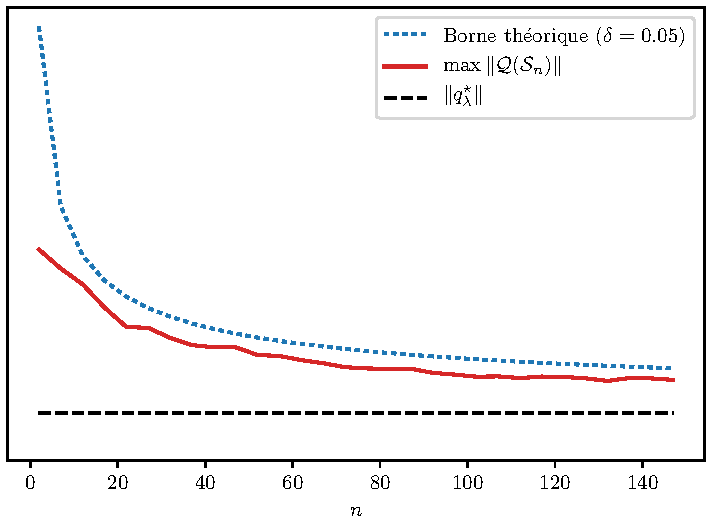
\includegraphics[width=0.7\textwidth]{../../experiments/fig/normqhqsl.pdf}
%   \caption{Illustration du \lemref{b:lem:qhnorm}.}
%   \label{fig:normqhqsl}
% \end{figure}
% \end{numex}


\begin{lemme}
  La solution $\qh_1$ de
  \begin{equation}
    \maximizeEquation[q \in \Q]{\EN_\lambda(q) = \hE\braket{q|t} - \tfrac{\lambda}{2}\|q\|^2.}
  \end{equation}
  est donnée par
  \begin{equation}
    \bra{\qh_1} = \lambda^{-1}\hE\bra{t}
  \end{equation}
  où $\bra{x_i} = \kappa(x_i,\cdot)$ est l'élément dual de $x$ sous $\Q$. Sous un noyau linéaire cela
  revient donc à 
  \begin{equation}
    \qh_1^T = \lambda^{-1}\hat\E(r^Tx)
  \end{equation}
  c'est à dire la covariance décentrée entre $r$ et $x$. On observera aussi que
  \begin{equation}
    \EN = \lambda\braket{\qh_1|\cdot}.
  \end{equation}
  et donc que
  \begin{equation}
    \EN(\qh_1) = \lambda\|\qh_1\|^2.
  \end{equation}
\end{lemme}

\begin{proof}
  Si on considère un déplacement de décision $\qh_1 + \Delta q$, alors par linéarité le premier
  terme de l'objectif devient $\EN(\qh_1+\Delta q) = \EN(\qh_1) + \EN(\Delta q)$ et le terme de
  régularisation devient 
  \begin{equation}
    -\lambda/2\|\qh_1 + \Delta q\|^2 = -\lambda/2\|\qh_1\|^2 - \lambda\braket{\qh_1|\Delta q} - \lambda/2\|\Delta q\|^2.
  \end{equation}
  On a donc
  \begin{align}
    \EN_\lambda(\qh_1)  - \EN_\lambda(\qh_1+\Delta q) &= -\EN(\Delta q) + \lambda\braket{\qh_1|\Delta q} + \lambda/2\|\Delta q\|^2\\
                                     &= -\lambda\braket{\qh_1|\Delta q} + \lambda\braket{\qh_1|\Delta q} +
                                       \lambda/2\|\Delta q\|^2\\
                                     &= \lambda/2\|\Delta q\|^2 \geq 0,
  \end{align}
  Ce qui entraîne $\EN_\lambda(\qh_1) \geq \EN_\lambda(\qh_1 + \Delta q)$.
\end{proof}

\begin{lemme}[Borne sur la décision utilitaire]
  \label{lem:rn}
  Pour toute fonction d'utilité $u$ respectant les hypothèses,
  \begin{equation}
    \|\qh_1\| \geq \|\qh_u\|.
  \end{equation}
  Ce lemme entraîne notamment que l'utilité en échantillon $\hEU(\qh_u) \leq \hEN(\qh_1)$:
  puisque $u(x) \leq x$,
  \begin{align}
    \hEU(\qh_u)&\leq \hEN(\qh_u) = \lambda\braket{\qh_1,\qh_u} \leq \lambda\|\qh_1\|\|\qh_u\| \leq \lambda\|\qh_1\|^2\\
               &=  \hEN(\qh_1)
  \end{align}
\end{lemme}

\begin{proof}
  On note tout d'abord avec l'inégalité de Jensen que
  $u(\hEN(\qu)) \geq \hEU(\qu) \geq \lambda/2\|\qu\|^2 \geq 0$ puisque la valeur de l'objectif
  $\hEN_\lambda(q)$ est d'au moins 0 à $q=0$. Mais puisque $u$ a un sur-gradient de 1 à
  $0$, on déduit que $u(x) \geq 0$ entraîne $x \geq u(x)$. On a ainsi
  $\hEN(\qu) - \lambda/2\nq{\qu}^2 \geq 0$. Ce qui entraîne alors que
  \begin{equation}
    \lambda\braket{\qh_1|\qh_u} \geq \lambda/2\|\qh_u\|^2
  \end{equation}
  Mais par Cauchy-Schwartz, on a aussi
  \begin{equation}
    \|\qh_1\|\|\qh_u\| \geq \braket{\qh_1,\qh_u} \geq \|\qh_u\|^2/2
  \end{equation}
  Et donc
  \begin{equation}
    \|\qh_1\| \geq \|\qh_u\|/2.\qedhere
  \end{equation}
\end{proof}


\begin{lemme}
L'erreur de généralisation du problème averse au risque est bornée par celle du problème
neutre au risque:
\begin{equation}
  \hEU(\qu) - \EU(\qu) \leq \gamma(\hEN(\qn) - \EN(\qn)).
\end{equation}
\end{lemme}
\begin{proof}
  Puisque $u$ est monotone, on peut tout d'abord noter que pour tout $r+\Delta \in \R$, on a
  l'inégalité $u(r+\Delta) \leq u(r) + \Delta \partial u(r)$. Ainsi, pour deux variables aléatoires $R_1,R_2 \in
  \R$, en posant $\Delta = R_1-R_2$, on a nécessairement
  \begin{equation}
    u(R_1) - u(R_2) \leq \partial u(R_2) (R_1 -R_2) \leq \gamma(R_1 - R_2),
  \end{equation}
  par définition du coefficient Lipschitz. On tire donc
  \begin{equation}
    \E u(R_1) - \E u(R_2) \leq \gamma(\E R_1 - \E R_2). 
  \end{equation}
  En appliquant cette inégalité aux opérateurs $\hEU$ et $\EU$ on obtient alors
  \begin{align}
    \hEU(\qu) - \EU(\qu) &\leq \gamma(\hEN(\qu) - \EN(\qu))\\
                         &= \gamma\lambda(\braket{\qh_1|\qu} - \braket{\qsl|\qu}).
  \end{align}
  Mais par le \lemref{lem:rn}, $\braket{\qh_1|\qu} \geq 0$ et $\|\qu\| \leq 2\|\qh_1\|$. 
\end{proof}



%%% Local Variables:
%%% mode: latex
%%% TeX-master: "memoire"
%%% End:
